% Created 2023-12-26 mar 15:58
% Intended LaTeX compiler: pdflatex
\documentclass[11pt]{article}
\usepackage[utf8]{inputenc}
\usepackage[T1]{fontenc}
\usepackage{graphicx}
\usepackage{grffile}
\usepackage{longtable}
\usepackage{wrapfig}
\usepackage{rotating}
\usepackage[normalem]{ulem}
\usepackage{amsmath}
\usepackage{textcomp}
\usepackage{amssymb}
\usepackage{capt-of}
\usepackage{hyperref}
\author{Claudio Vaucheret}
\date{Planificación: POP}
\title{Inteligencia Artificial}
\hypersetup{
 pdfauthor={Claudio Vaucheret},
 pdftitle={Inteligencia Artificial},
 pdfkeywords={},
 pdfsubject={},
 pdfcreator={Emacs 27.1 (Org mode 9.4)}, 
 pdflang={English}}
\begin{document}

\maketitle
\setcounter{tocdepth}{1}
\tableofcontents


\section*{Repaso}
\label{sec:org8b1ed71}

\subsection*{¿Qué vimos?}
\label{sec:orgee194eb}
\begin{itemize}
\item Representación de las acciones: STRIPS, Situation Calculus, Event Calculus
\item Problemas en la representación del Cambio: Frame, Ramification y Qualification
\item Regresión
\item PLanning
\end{itemize}


{\color{red}HOY}
{\color{red}Algoritmos de Planificación: Planificador de Orden Parcial}

\section*{Planificación de Orden Parcial}
\label{sec:orga9854a9}

\subsection*{Planificación de Orden Parcial}
\label{sec:org2fc595e}
\begin{itemize}
\item Los planificadores dados dan como resultado un plan  totalmente ordenado.
\item No utilizan las ventajas de la descomposición del problema.
\item Al utilizar un orden parcial entre acciones sólo se compromete un
orden sobre las acciones cuando realmente fuere necesario.
\end{itemize}

\subsection*{Back to Matemática Discreta :)}
\label{sec:org1661dbd}

{\color{red}¿Qué es un orden parcial?}
Es una relación de orden reflexiva, antisimétrica y transitiva.

{\color{red}¿y un orden parcial estricto?}
Un orden parcial estricto es irreflexivo, transitivo y asimétrico.

Utilizaremos para el orden parcial la relación {\color{red}antes que},
que es irreflexiva, asimétrica y transitiva, es decir es un
{\color{red}orden parcial estricto}.

\subsection*{Back to the future: IA}
\label{sec:orgb4147e4}
\begin{itemize}
\item \textbf{{\color{green}Planificación de Orden Parcial}}
\begin{itemize}
\item un conjunto de {\color{red}acciones} junto con un {\color{red}orden parcial},
representando la relación {\color{blue}antes que} sobre acciones,
\item cualquier orden total sobre las acciones, consistente con el
orden parcial, resuelve la meta desde el nodo inicial
\end{itemize}
\item Si tenemos el siguiente orden parcial entre las acciones:
\begin{itemize}
\item \(a_1 < a_2\)  \(a_3 < a_4\)
\item los siguientes órdenes totales son {\color{red}consistentes} con el orden parcial anterior:
\begin{itemize}
\item \(a_1 < a_2 < a_3 < a_4\) , \(a_3 < a_4 < a_1 < a_2\)
\item \(a_3 < a_1 < a_4 < a_2\) , \(a_1 < a_3 < a_4 < a_2\)
\end{itemize}
\end{itemize}
\end{itemize}

\subsection*{Zapatos y Medias}
\label{sec:orgbe0588f}

\begin{itemize}
\item \textbf{{\color{green}Zapatos y Medias}}
\begin{itemize}
\item Supongamos que quiero ponerme los zapatos y las medias en ambos pies. Hagamos un plan para esto.
\item Una solución:
\begin{itemize}
\item MediaIzq- MediaDer-ZapDer-ZapIzq      

¿Otra solución?
\end{itemize}
\end{itemize}
\end{itemize}


\subsection*{Zapatos y Medias}
\label{sec:org8d18f41}

\begin{itemize}
\item \textbf{{\color{green}Orden Parcial}}
\begin{itemize}
\item {\color{red}MedDer \(<\) ZapDer}
\item {\color{red}MedIzq \(<\) ZapIzq}
\end{itemize}
\item Cualquier orden total consistente con este orden parcial estricto
es solución al problema.
\end{itemize}




\subsection*{Orden entre las Acciones}
\label{sec:org6ef2727}

\begin{itemize}
\item \textbf{{\color{green}\(A_0 < A_1\)}}
\begin{itemize}
\item La acción \(A_0\)  está antes que \(A_1\) en el orden parcial.
\item La acción \(A_0\)  ocurrió antes que \(A_1\).
\end{itemize}
\item \textbf{{\color{green}¡Atención!}}
\begin{itemize}
\item \(A_0\)  {\color{red}no} es necesario que esté inmediatamente antes que \(A_1\)
\end{itemize}
\end{itemize}



\subsection*{Acciones Especiales}
\label{sec:org00a47f4}
\begin{itemize}
\item \textbf{{\color{green}START}}
\begin{itemize}
\item Es una acción que alcanza las relaciones que son verdaderas en
el estado inicial. Sin precondición y su efecto es agregar los
fluentes que son Verdaderos en el estado inicial.
\end{itemize}
\item \textbf{{\color{green}FINISH}}
\begin{itemize}
\item Es una acción cuyas precondiciones son las metas a ser
resueltas y no tiene efecto.
\end{itemize}
\item Son acciones que sirven al momento de construir el plan como límites.
\begin{itemize}
\item Cuando se ejecuta el plan START y FINISH son ignorados.
\end{itemize}
\end{itemize}



\subsection*{Acciones Especiales}
\label{sec:org1462794}

Para toda acción \(A\) se cumple que: 

\[START< A\]
\[A< FINISH\]
\[START< FINISH\]

\subsection*{Enlace Causal}
\label{sec:org2074196}

Para cada precondición \(P\) de la acción \(A_1\) tenemos asociada una  acción \(A_0\):

\begin{center}
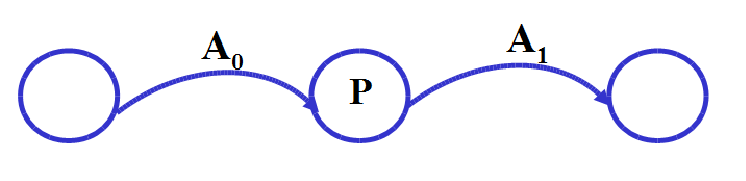
\includegraphics[width=.9\linewidth]{imagenes/EnlaceCausal.png}
\end{center}

\[A_0\ <\ A_1\]

\subsection*{Enlace Causal}
\label{sec:org513fecc}

Cada acción \(A\) que borre a \(P\) tiene que estar antes de \(A_0\) o
después de \(A_1\):

\begin{center}
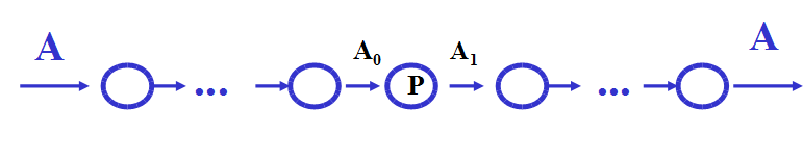
\includegraphics[width=.9\linewidth]{imagenes/EnlaceCausal2.png}
\end{center}

   \[A_0\ <\ A_1\ <\ A\]
o bien 

\[A\ <\ A_0\ <\ A_1\]

\subsection*{Enlace Causal}
\label{sec:org75c2b4f}
\begin{itemize}
\item \textbf{{\color{green}Enlace Causal}}
\begin{itemize}
\item Es un término de la forma {\color{red}\(cl(A_0,P,A_1)\)} donde
\(A_0\) y \(A_1\) son acciones y \(P\) es un fluente. \(P\) es una
precondición de la acción \(A_1\). La acción \(A_0\) logra \(P\). \(P\)
está soportado por la acción \(A_0\).
   \begin{center}
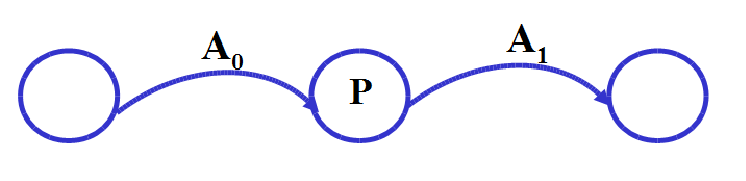
\includegraphics[width=.9\linewidth]{imagenes/EnlaceCausal.png}
\end{center}
\end{itemize}
\item \textbf{{\color{green}Amenaza}}
\begin{itemize}
\item Una acción \(A\) {\color{red}amenaza} un enlace causal \(cl(A_0,P,A_1)\) si la
acción \(A\) borra la proposición \(P\).
\end{itemize}
\end{itemize}



\subsection*{Amenaza del enlace causal}
\label{sec:orgc61948e}
\begin{itemize}
\item \textbf{{\color{green}Amenaza}}
\begin{itemize}
\item Una acción \(A\)  {\color{red}amenaza} un enlace causal
\(cl(A_0,P,A_1)\) si la acción \(A\) borra la proposición \(P\).
\end{itemize}
\end{itemize}

Para resolver las amenazas,
se añaden restricciones de orden:
Nos aseguramos de que la acción
que amenaza (s3) no interviene
en el enlace causal (de s1 a s2)


\begin{center}
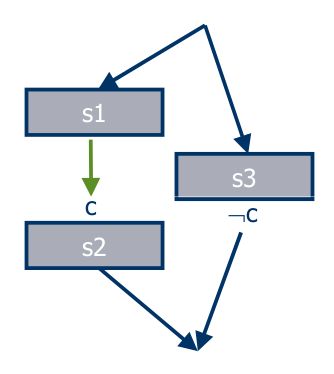
\includegraphics[width=.9\linewidth]{imagenes/amenazaCausal.png}
\end{center}

\subsection*{Amenaza del enlace causal}
\label{sec:org7cebfff}
\begin{itemize}
\item \textbf{{\color{green}Dos formas de resolver amenazas}}:
\begin{itemize}
\item \textbf{Degradación:} La acción que amenaza se realiza antes del vínculo causal.
\item \textbf{Ascenso:} La acción que amenaza se realiza después del vínculo causal.
\end{itemize}
\end{itemize}
\begin{center}
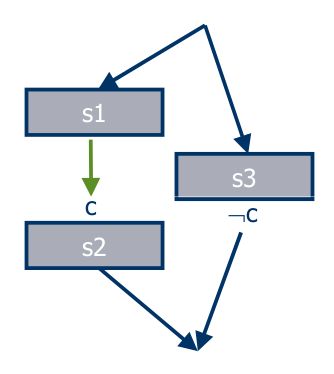
\includegraphics[width=.9\linewidth]{imagenes/amenazaCausal.png}
\end{center}

\subsection*{Amenaza del enlace causal}
\label{sec:orga9faba1}
\begin{center}
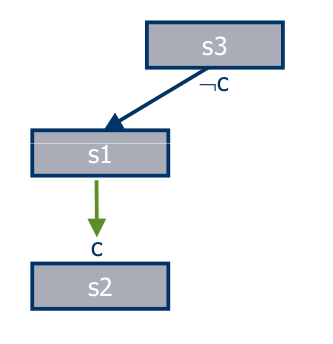
\includegraphics[width=.9\linewidth]{imagenes/arriba.png}
\end{center}

\begin{center}
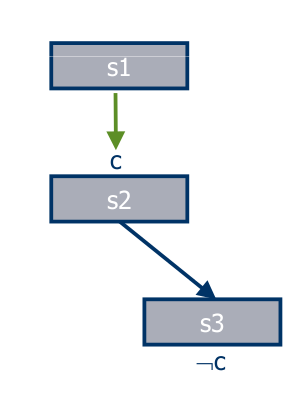
\includegraphics[width=.9\linewidth]{imagenes/abajo.png}
\end{center}



\subsection*{Amenaza del enlace causal}
\label{sec:org4866c1c}

\begin{itemize}
\item Estas amenazas no se pueden resolver directamente (las dos
acciones se amenazan mutuamente y ningún orden permite
resolverlas).
\end{itemize}

\begin{center}
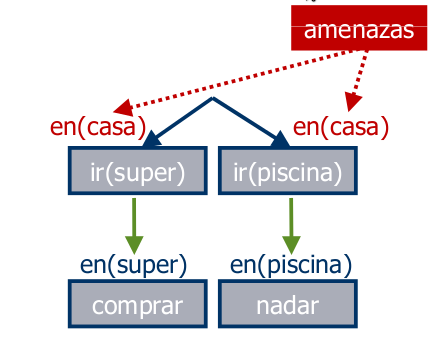
\includegraphics[width=.9\linewidth]{imagenes/casa.png}
\end{center}

\subsection*{Amenaza del enlace causal}
\label{sec:orga432f42}

\begin{center}
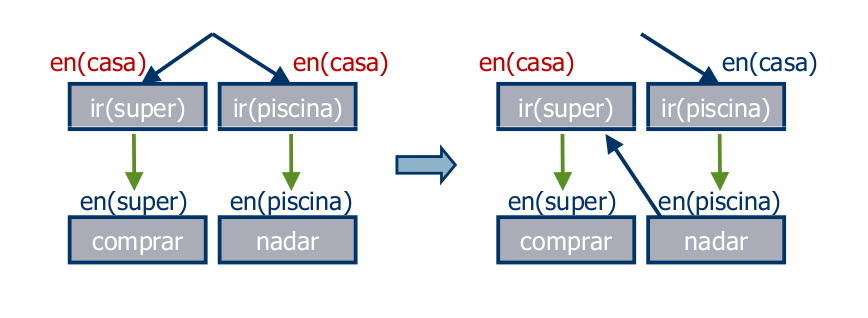
\includegraphics[width=.9\linewidth]{imagenes/solcasa.png}
\end{center}

\subsection*{Plan de Orden Parcial}
\label{sec:org3fb5109}

\begin{itemize}
\item \textbf{{\color{green}Plan Parcial}}
\begin{itemize}
\item Un {\color{red}plan parcial} es un término de la forma
\(plan(As,Os,Ls)\), donde \(As\) es una lista de acciones, \(Os\) es
un orden parcial sobre acciones y \(Ls\) es una lista de enlaces
causales.
\end{itemize}
\item \textbf{{\color{green}Plan Seguro}}
\begin{itemize}
\item El plan es {\color{red}seguro} si para toda acción \(A\in As\)
que amenaza a \(cl(A_0,P,A_1)\in Ls\) , el orden parcial \(Os\)
deriva que \(A< A_0\) o \(A_1 < A\).
\end{itemize}
\end{itemize}

\subsection*{Plan de Orden Parcial}
\label{sec:org8f7bd1f}

\begin{itemize}
\item \textbf{{\color{green}Agenda}}
\begin{itemize}
\item Una {\color{red}agenda} es un conjunto de submetas para cada
precondición no soportada de todas las metas en \(As\).
\end{itemize}
\item \textbf{{\color{green}Submeta}}
\begin{itemize}
\item Una {\color{red}submeta} es un término de la forma {\color{red}goal(P,A)}, donde \(P\) es
una proposición atómica que es una precondición para la acción
\(A\).
\end{itemize}
\item \textbf{{\color{green}Plan Completo}}
\begin{itemize}
\item Un {\color{red}plan completo} es un plan parcial seguro con una
agenda vacía.
\end{itemize}
\end{itemize}





\subsection*{Planificador de Orden Parcial}
\label{sec:org53310ff}

\begin{center}
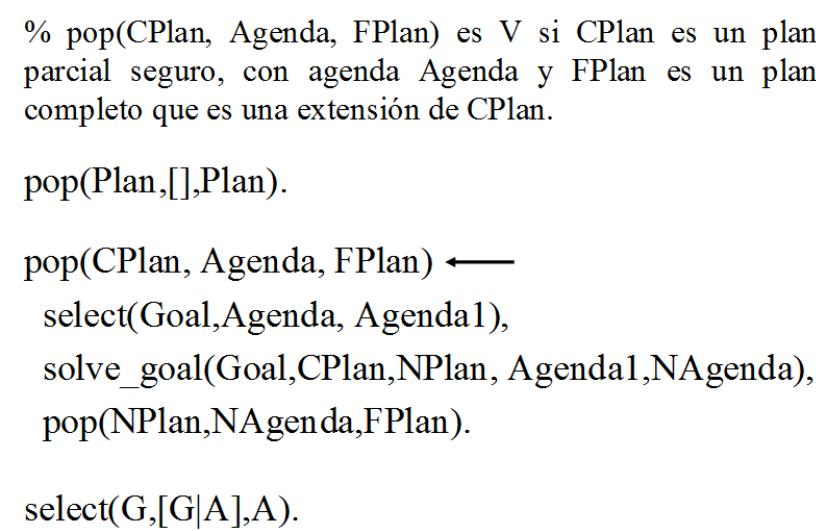
\includegraphics[width=.9\linewidth]{imagenes/Pop.png}
\end{center}

\subsection*{Planificador de Orden Parcial}
\label{sec:org8777bab}

\begin{center}
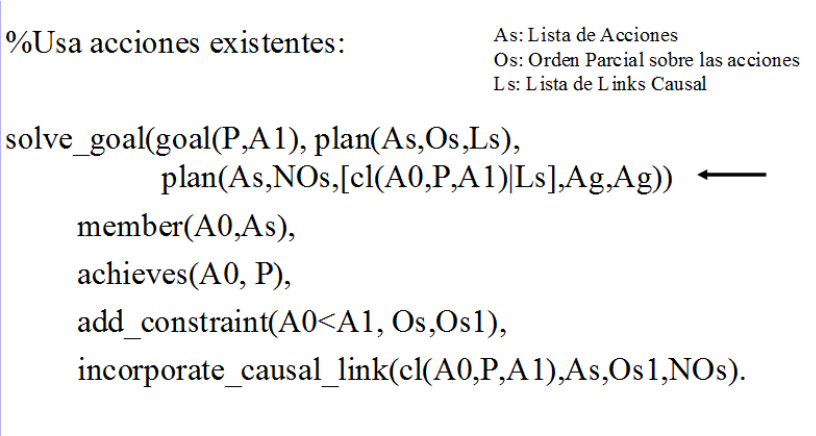
\includegraphics[width=.9\linewidth]{imagenes/Pop2.png}
\end{center}

\subsection*{Planificador de Orden Parcial}
\label{sec:org756563a}

\begin{center}
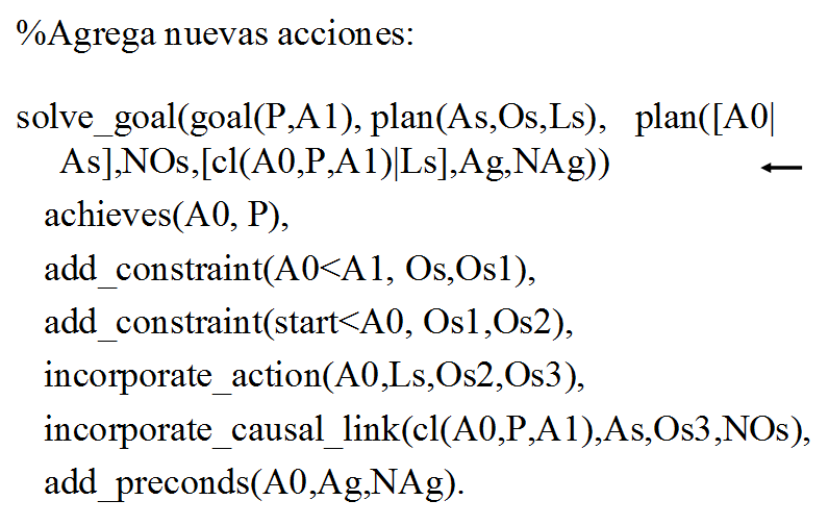
\includegraphics[width=.9\linewidth]{imagenes/Pop3.png}
\end{center}

\subsection*{Planificador de Orden Parcial}
\label{sec:orga6b2899}

\begin{center}
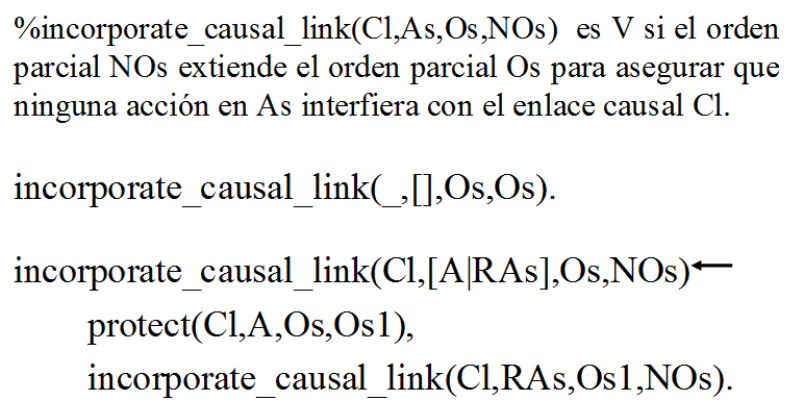
\includegraphics[width=.9\linewidth]{imagenes/Pop4.png}
\end{center}

\subsection*{Planificador de Orden Parcial}
\label{sec:org53cdc04}

\begin{center}
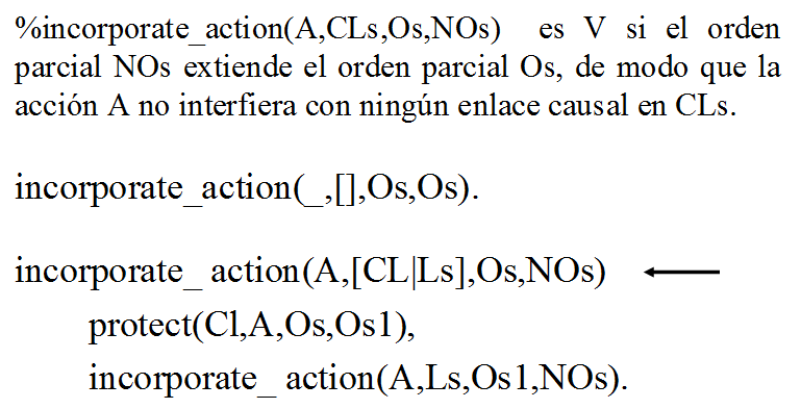
\includegraphics[width=.9\linewidth]{imagenes/Pop5.png}
\end{center}

\subsection*{Planificador de Orden Parcial}
\label{sec:org3613b2b}

\begin{center}
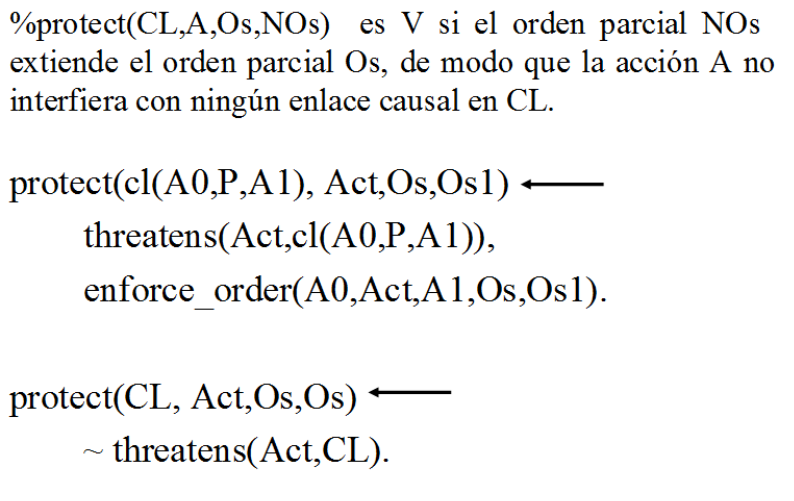
\includegraphics[width=.9\linewidth]{imagenes/Pop6.png}
\end{center}

\subsection*{Planificador de Orden Parcial}
\label{sec:org58d26d8}

\begin{center}
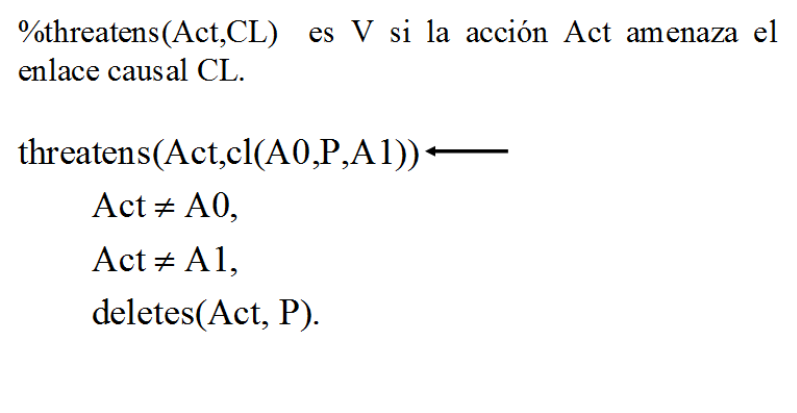
\includegraphics[width=.9\linewidth]{imagenes/Pop7.png}
\end{center}

\subsection*{Planificador de Orden Parcial}
\label{sec:orgc80e6e2}

\begin{center}
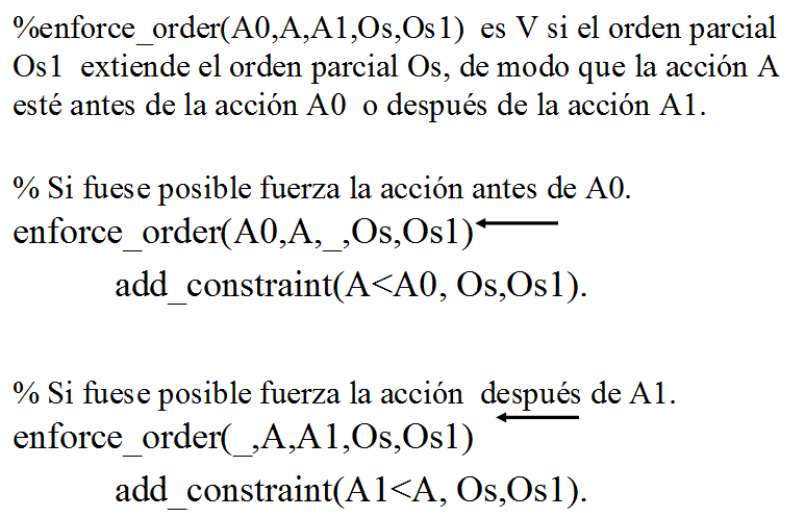
\includegraphics[width=.9\linewidth]{imagenes/Pop8.png}
\end{center}

\subsection*{Ejemplo}
\label{sec:org7c417ec}

\begin{center}
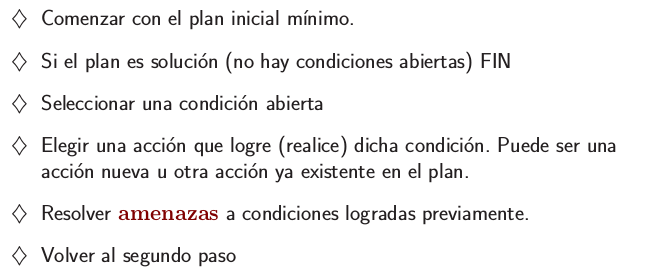
\includegraphics[width=.9\linewidth]{imagenes/poppseudo.png}
\end{center}

\subsection*{Ejemplo}
\label{sec:org7e6879e}

\begin{center}
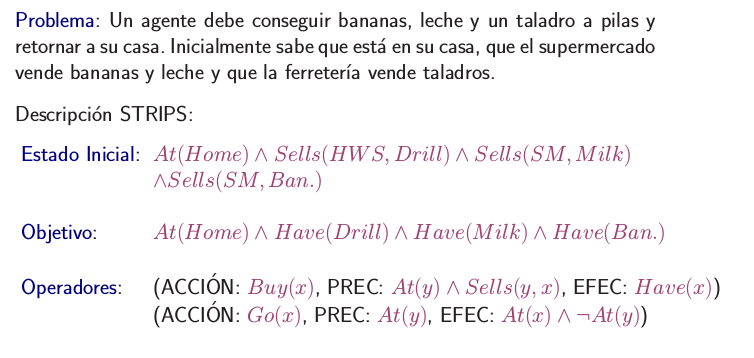
\includegraphics[width=.9\linewidth]{imagenes/pop0.png}
\end{center}

\subsection*{Ejemplo}
\label{sec:orgd842d81}

\begin{center}
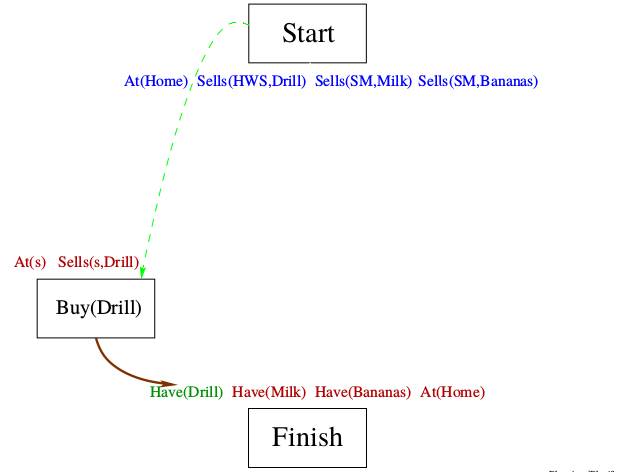
\includegraphics[width=.9\linewidth]{imagenes/pop2.png}
\end{center}

\subsection*{Ejemplo}
\label{sec:org72382f9}

\begin{center}
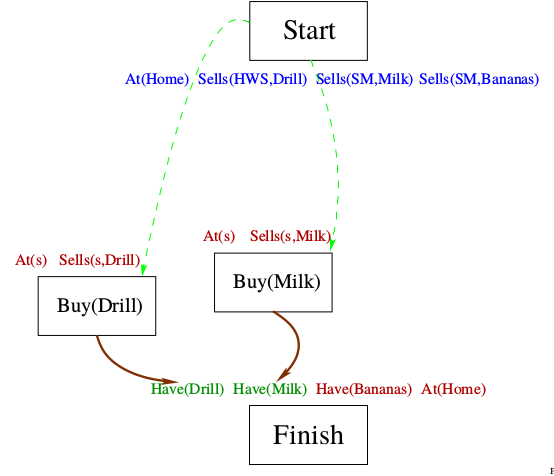
\includegraphics[width=.9\linewidth]{imagenes/pop4.png}
\end{center}

\subsection*{Ejemplo}
\label{sec:org97ebd84}

\begin{center}
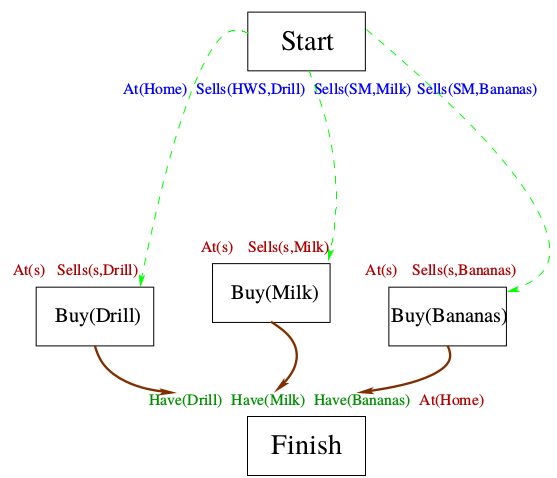
\includegraphics[width=.9\linewidth]{imagenes/pop5.png}
\end{center}

\subsection*{Ejemplo}
\label{sec:orgb4dad5c}

\begin{center}
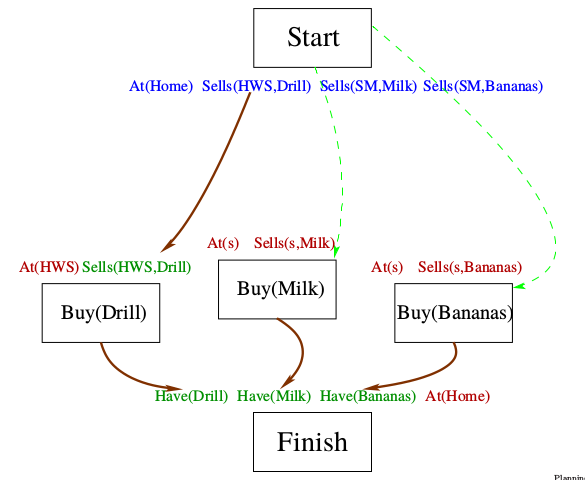
\includegraphics[width=.9\linewidth]{imagenes/pop6.png}
\end{center}

\subsection*{Ejemplo}
\label{sec:org51cfdde}

\begin{center}
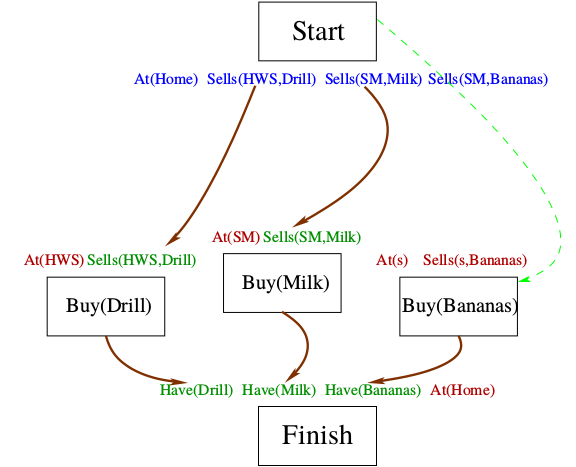
\includegraphics[width=.9\linewidth]{imagenes/pop7.png}
\end{center}

\subsection*{Ejemplo}
\label{sec:org34418da}

\begin{center}
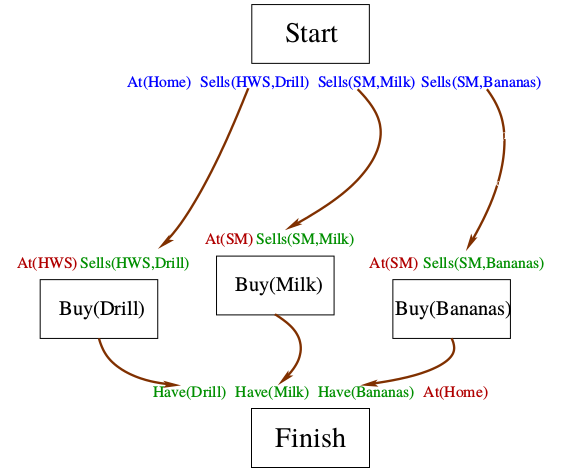
\includegraphics[width=.9\linewidth]{imagenes/pop8.png}
\end{center}

\subsection*{Ejemplo}
\label{sec:org156194c}

\begin{center}
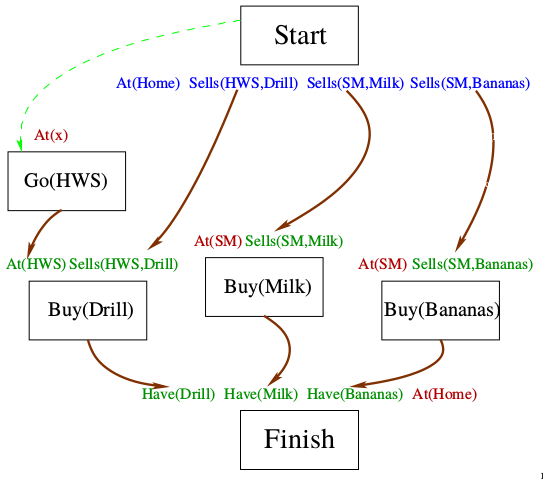
\includegraphics[width=.9\linewidth]{imagenes/pop9.png}
\end{center}

\subsection*{Ejemplo}
\label{sec:org1fb4f4b}

\begin{center}
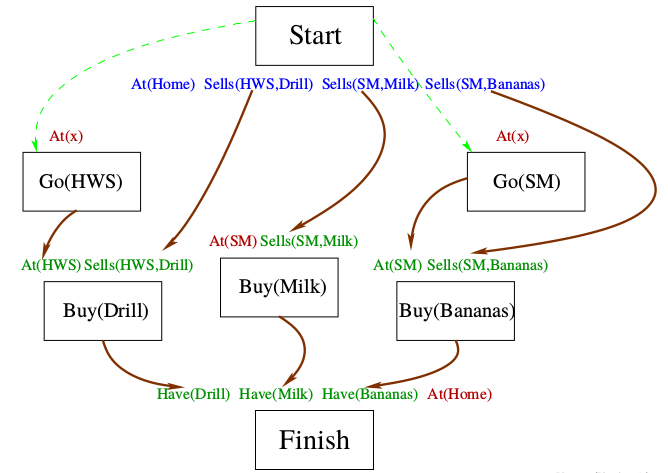
\includegraphics[width=.9\linewidth]{imagenes/pop10.png}
\end{center}

\subsection*{Ejemplo}
\label{sec:org40842fc}

\begin{center}
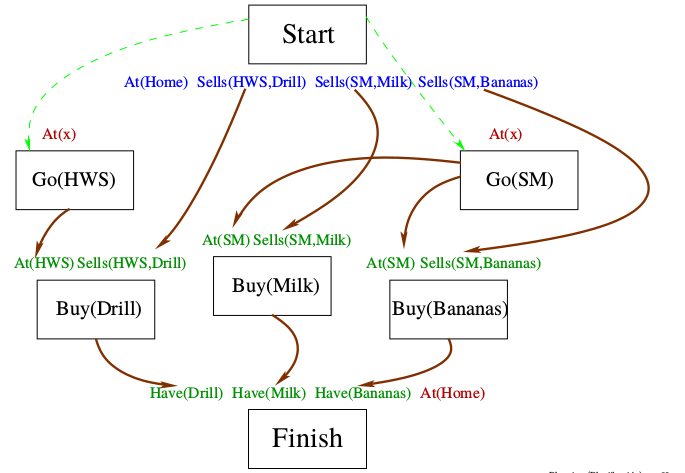
\includegraphics[width=.9\linewidth]{imagenes/pop11.png}
\end{center}

\subsection*{Ejemplo}
\label{sec:orgab0f0ee}

\begin{center}
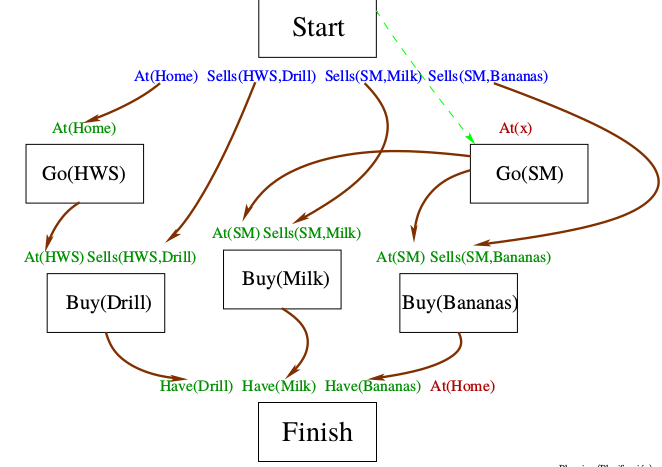
\includegraphics[width=.9\linewidth]{imagenes/pop12.png}
\end{center}

\subsection*{Ejemplo}
\label{sec:org441b86a}

\begin{center}
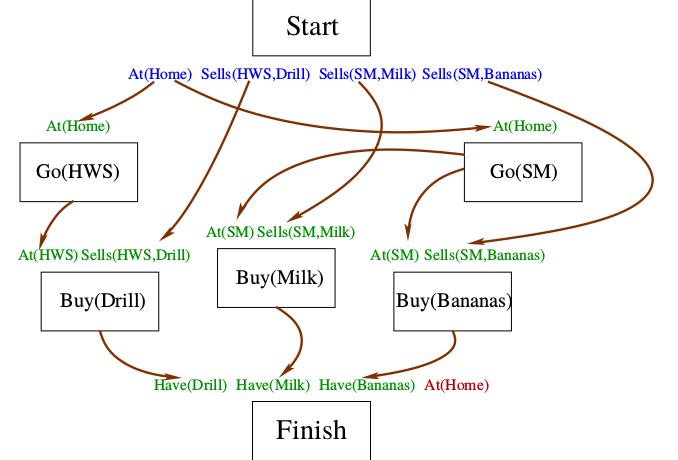
\includegraphics[width=.9\linewidth]{imagenes/pop15.png}
\end{center}

\subsection*{Ejemplo}
\label{sec:org8ba6de2}

\begin{center}
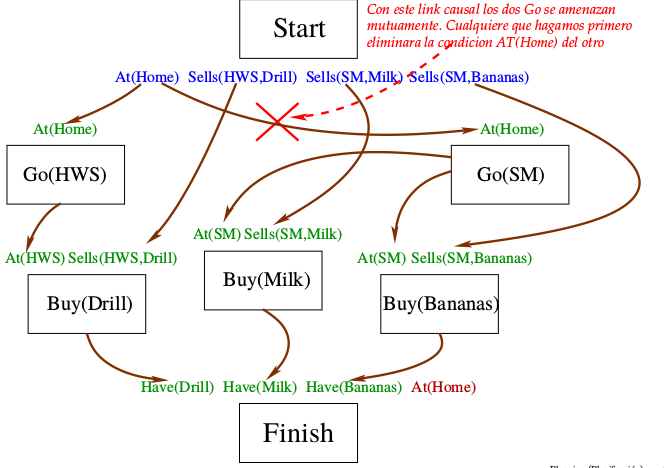
\includegraphics[width=.9\linewidth]{imagenes/pop16.png}
\end{center}

\subsection*{Ejemplo}
\label{sec:org73c4c61}

\begin{center}
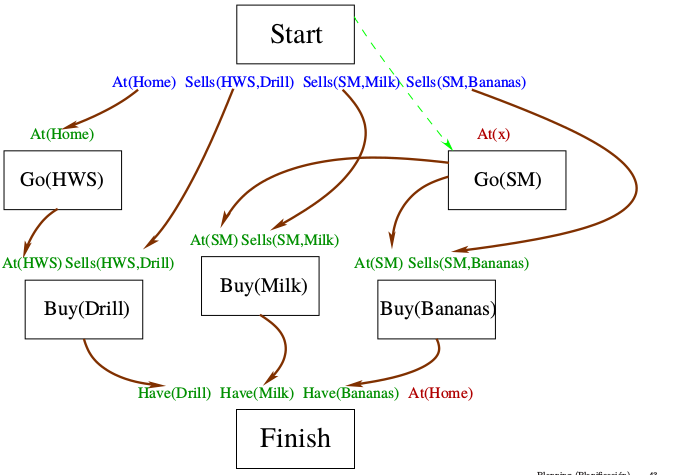
\includegraphics[width=.9\linewidth]{imagenes/pop17.png}
\end{center}

\subsection*{Ejemplo}
\label{sec:org9e706a0}

\begin{center}
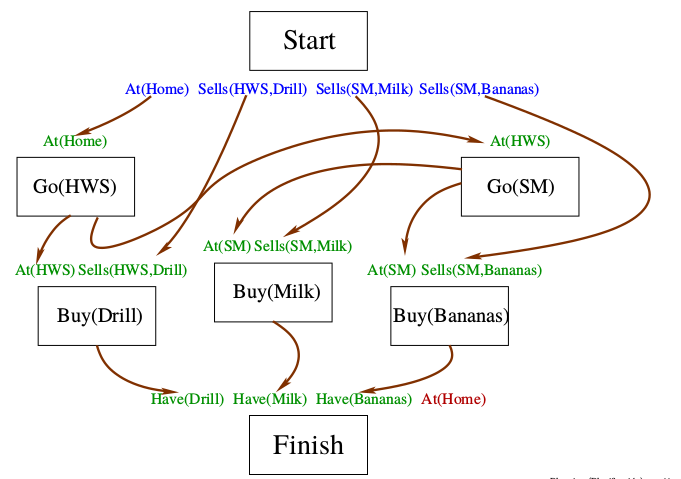
\includegraphics[width=.9\linewidth]{imagenes/pop18.png}
\end{center}

\subsection*{Ejemplo}
\label{sec:orgf38862b}

\begin{center}
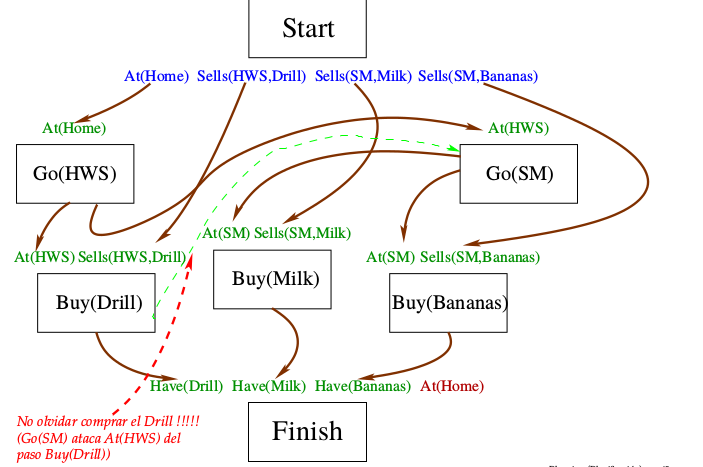
\includegraphics[width=.9\linewidth]{imagenes/pop19.png}
\end{center}

\subsection*{Ejemplo}
\label{sec:orgf61fe6f}

\begin{center}
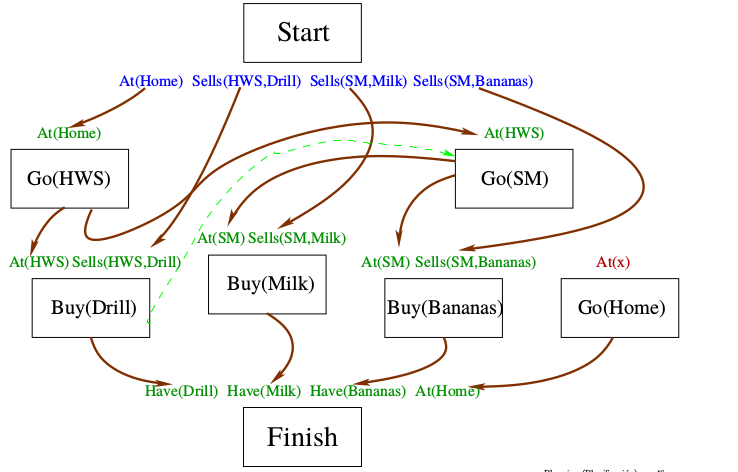
\includegraphics[width=.9\linewidth]{imagenes/pop20.png}
\end{center}

\subsection*{Ejemplo}
\label{sec:org2e1a46a}

\begin{center}
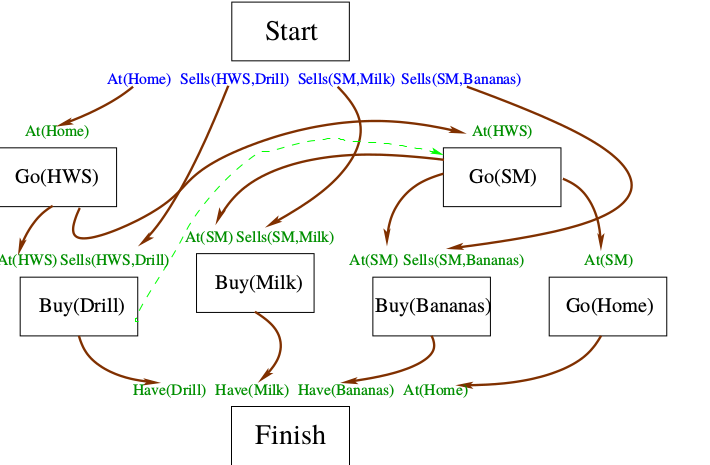
\includegraphics[width=.9\linewidth]{imagenes/pop21.png}
\end{center}

\subsection*{Ejemplo}
\label{sec:orga8a0f38}

\begin{center}
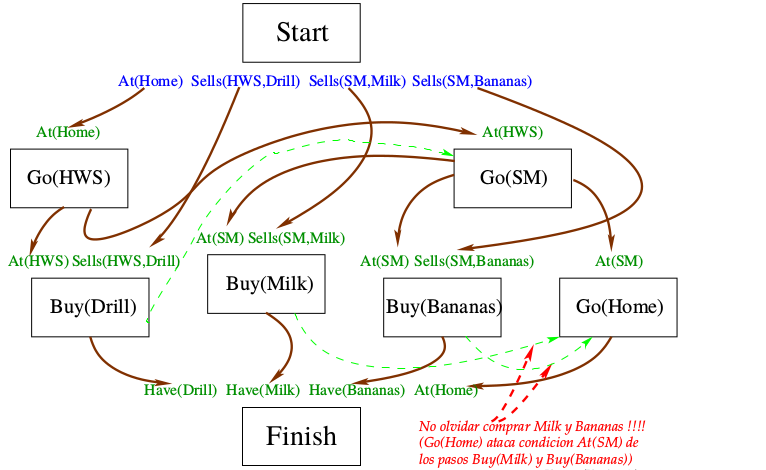
\includegraphics[width=.9\linewidth]{imagenes/pop23.png}
\end{center}

\subsection*{Ejemplo}
\label{sec:org662d4e8}

\begin{center}
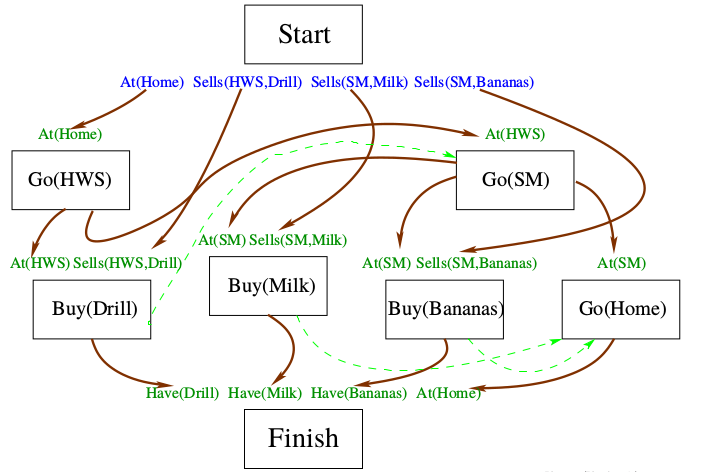
\includegraphics[width=.9\linewidth]{imagenes/pop24.png}
\end{center}

\subsection*{Ejemplo}
\label{sec:org1fb8e56}

\begin{center}
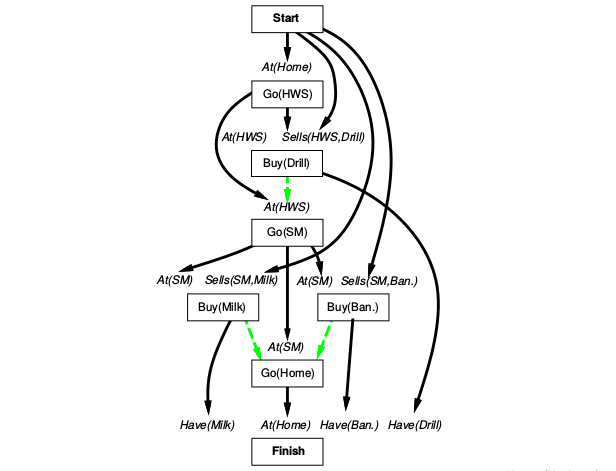
\includegraphics[width=.9\linewidth]{imagenes/pop25.png}
\end{center}
\end{document}